\documentclass[12pt, french]{article}

\usepackage{fancyhdr, fancybox, lastpage}
\usepackage[most]{tcolorbox}
\usepackage[a4paper, margin={0.3in, .75in}]{geometry}
\usepackage{wrapfig}
\pagestyle{fancy}
\renewcommand\headrulewidth{1pt}
\renewcommand\footrulewidth{1pt}
\fancyhf{}
\rhead{ \em{Zakaria Haouzan}}
\lhead[C]{\em{2ème année baccalauréat Sciences Mathématiques}}
\chead[C]{}
\rfoot[C]{}
\lfoot[R]{}
\cfoot[]{\em{Page \thepage / \pageref{LastPage}}}


\newtcolorbox{Box2}[2][]{
                lower separated=false,
                colback=white,
colframe=white!20!black,fonttitle=\bfseries,
colbacktitle=white!30!gray,
coltitle=black,
enhanced,
attach boxed title to top left={yshift=-0.1in,xshift=0.15in},
title=#2,#1}


\begin{document}
\begin{center}
   \shadowbox {\bf{Les Ondes Mécaniques Progressives }}
\end{center}

\vspace{-0.2cm}
%%_________________________Exercice ! :"_________________________Exercice
   \begin{Box2}{Exercice 1 :  la propagation d’une onde le long d’une corde}

La figure ci-dessous représente la propagation d’une onde le long d’une corde. Elle représente l’aspect de la
corde à l’instant $t = 40ms$. Sachant que la déformation commence à partir d’une source à l’instant $t_0 =0$.
   \begin{center}
	   \vspace{-0.6cm}
	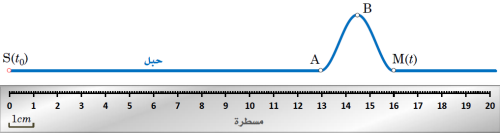
\includegraphics[width=0.6\textwidth ]{./img/Exercice01.png}
  \end{center}
1. Définir une onde mécanique progressive.

2. Quelle la nature de l’onde ? quelle est sa dimension ?

3. Déterminer, à l’instant t, les points qui se dirigeront vers le bas ainsi que ceux se dirigeront vers le haut.

4. Calculer V la célérité de la propagation de l’onde le long de la corde.

5. A quel instant s’arrête le point M (position du début de la propagation).

6. Représenter graphiquement l’aspect de la corde à l’instant t’=10ms.

7. Déterminer la relation entre l’élongation du point M et celle de la source S.


   \end{Box2}


%%_________________________Exercice !2 :"_________________________Exercice
\begin{Box2}{Exercice 2 :  retard temporaire }
\begin{wrapfigure}{r}{0.22\textwidth}
  \begin{center}
	  \vspace{-0.6cm}
	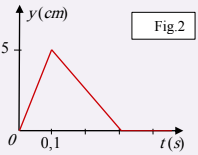
\includegraphics[width=0.22\textwidth]{./img/Ex2.png}
  \end{center}
\end{wrapfigure}
Une perturbation se propage, à partir de la source S , le long d’une corde élastique avec une célérité $v$=$10m/s$.
Le schéma de la Fig.2 représente la variation de l’élongation de la source en fonction du temps.
On considère un point M de la corde situé à 4m de la source.

1. Déterminer la durée de la perturbation.

2. Calculer le retard du point M par rapport au point S.

3. Représenter la variation de l’élongation du point M en fonction du temps.

\end{Box2}

%%_________________________Exercice ! 3:"_________________________Exercice
\begin{Box2}{Exercice 3 :Vitesse de propagation d’une onde }
\begin{wrapfigure}{r}{0.38\textwidth}
  \begin{center}
	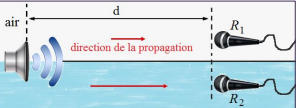
\includegraphics[width=0.38\textwidth]{./img/Ex3.png}
  \end{center}
\end{wrapfigure}
Dans un bassin d’essais, une source sonore S émet un bruit intense qui se propage dans l’air et dans l’eau. Le bruit est reçu par deux récepteurs sonores: $R_1$ placé dans l’air et $R_2$ situé dans l’eau

\underline{Données: célérité du son }
\begin{itemize}
	\item Dans l’air: $V_{air} = 340m/s$
	\item Dans l’eau: $V_{eau} = 1500m/s$
\end{itemize}
1.Quel est le récepteur qui, le premier, détecte le bruit produit par la source?

2.On note $\Delta{t}$ la durée séparant la détection du bruit par les récepteurs $R_1$ et $R_2$
Exprimer la distance d séparant la source des récepteurs en fonction de la durée $\Delta{t}$ et des célérités $V_{air}$ et $V_{eau}$.

3.Calculer la valeur de d pour $\Delta{t}$=$0.50s$
\end{Box2}

%%_________________________Exercice 4 : _________________________Exercice
\begin{Box2}{Exercice 4 :corde élastique }
\begin{wrapfigure}{r}{0.4\textwidth}
  \begin{center}
	  \vspace{-0.6cm}
	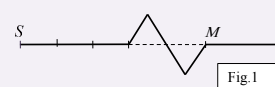
\includegraphics[width=0.4\textwidth]{./img/Ex4}
  \end{center}
\end{wrapfigure}
Une perturbation se propage le long d’une corde élastique de masse linéique $\mu$=$6,4g/m$, soumise  à une tension F=1N. S est l’extrémité de la corde, source de la
perturbation.

La fig.1 représente, avec une échelle 1/50,l’aspect de la corde à un instant $t_1$.

1. L’onde est-elle transversale ou longitudinale? Justifier votre réponse.

2. Calculer la célérité de l’onde.

3. Dessiner l’aspect de la corde à l’instant $t_2$=$t_1 + 0,1$ (s).

4. Pendant quelle durée un point de la corde est-il affectée par le passage de la perturbation?

5. Calculer la durée $\Delta{t}$ nécessaire pour que la perturbation parvienne au point M.


\end{Box2}
%\vspace{2cm}
\begin{center}
   \Large{ \em{Exercices Supplémentaires}}
\end{center}


\vspace{-0.7cm}
%%_________________________Exercice 5 : _________________________Exercice
\begin{Box2}{Exercice 5 :Les ondes sonores }
Pour mesurer la propagation des ondes sonores dans l’air on réalise le montage expérimental représentant ci-dessous, la distance entre les deux microphones R1 et R2 est d=1,70m. La courbe ci-dessous représente la variation de la tension aux bornes de chaque microphone.

\underline{Donnée : }La sensibilité horizontale : 1ms/div ; température d’air 25°C ; célérité de la propagation du son dans l’eau $V_{eau}$=$1500m/s$.


	\begin{center}
		\vspace{-0.5cm}
	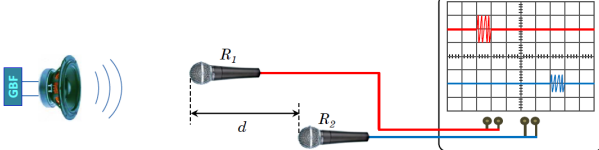
\includegraphics[width=0.7\textwidth]{./img/Ex5.png}
  \end{center}
1. Est que le son est une onde longitudinale ou transversale.

2. Déterminer la valeur du retard temporel entre les microphones R1 et R2.

3. Déduire la valeur Vair célérité de la propagation des ondes sonores dans l’air.

4. Déterminer la valeur du retard temporel $\tau'$ quand on déplace le microphone vers la droite à partir de sa position initiale de L= 51cm.

5. Comparer $V_{air}$ et $V_{eau}$. Que peut-t-on déduire.

\end{Box2}
%%_________________________Exercice 6 : _________________________Exercice
\begin{Box2}{Exercice 6 : échographie}
\begin{wrapfigure}{r}{0.2\textwidth}
  \begin{center}
	  \vspace{-0.6cm}
	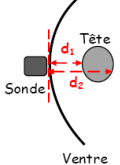
\includegraphics[width=0.2\textwidth]{./img/Exercice6.png}
  \end{center}
\end{wrapfigure}
	Lors d’une échographie d’un foetus, la sonde posée sur le ventre de la mère (voir schéma ci-dessous) émet et reçoit des signaux ultrasonores.

	L’ordinateur calcule la durée $\Delta{t}$ mis par le signal émis pour faire un aller jusqu’au foetus et un retour jusqu’au récepteur.

La vitesse v de propagation des ondes ultrasonores dans le corps humain est de $1500 m/s$.

La sonde orientée vers la tête du foetus reçoit un premier signal avec un décalage
$\Delta{t}$=$3,0.10^{-5}s$ après l’émission, et un deuxième signal avec $\Delta{t}$=$7,0.10^{-5}s$.

1. Calculer la distance $d_1$ entre la sonde et la paroi la plus proche de la tête du foetus.

2. Calculer la distance $d_2$ entre la sonde et la paroi la plus éloigné de la tête du foetus.

3. Déduire le diamètre d de la tête du foetus en cm.

\end{Box2}

\end{document}
